\documentclass[10pt,twocolumn]{article}

\usepackage[utf8]{inputenc}
\usepackage[T1]{fontenc}
\usepackage{lmodern}
\usepackage[margin=0.75in,top=0.85in,bottom=0.85in]{geometry}
\usepackage{amsmath,amssymb,amsfonts}
\usepackage{booktabs}
\usepackage{tabularx}
\usepackage{multirow}
\usepackage{graphicx}
\usepackage{xcolor}
\usepackage{tikz}
\usetikzlibrary{shapes.geometric, arrows.meta, positioning, fit, calc, backgrounds}
\usepackage{listings}
\usepackage{url}
\usepackage[colorlinks=true,linkcolor=blue!60!black,citecolor=blue!60!black,urlcolor=blue!60!black]{hyperref}

\definecolor{aegisblue}{RGB}{28, 78, 128}
\definecolor{aegisgreen}{RGB}{34, 139, 34}
\definecolor{aegisred}{RGB}{180, 40, 40}
\definecolor{aegisgray}{RGB}{245, 247, 250}
\definecolor{codebg}{RGB}{248, 249, 252}

\lstset{
  basicstyle=\ttfamily\scriptsize,
  backgroundcolor=\color{codebg},
  frame=single,
  rulecolor=\color{black!20},
  breaklines=true,
  columns=fullflexible,
  keepspaces=true,
  showstringspaces=false
}

\setlength{\columnsep}{0.25in}
\emergencystretch=1.5em

\title{\LARGE \textbf{Aegis OS: A Transactional Multi-Tenant Operating System Runtime for Eliminating Authorization Fatigue in Autonomous Coding Agents}}

\author{
  \textbf{Hui Zhao} \\
  \texttt{huizhao@heurion.org}
}

\date{Preprint --- October 2026}

\begin{document}

\maketitle

\begin{abstract}
Autonomous coding agents such as Google Antigravity (\texttt{agy}), Anthropic Claude Code (\texttt{claude}), and OpenAI Codex CLI (\texttt{codex}) increasingly execute complex, multi-step software engineering workflows directly on developer workstations and enterprise cloud hosts. However, existing agent execution environments suffer from a fundamental \emph{Security--Autonomy Dilemma}: users must choose between \emph{Interactive Per-Action Prompting}, which interrupts human operators on 43\%--60\% of tool invocations and induces severe authorization fatigue, or \emph{Unconfined Host Execution} (\texttt{--yolo} / \texttt{--dangerously-skip-permissions}), which exposes the host filesystem, SSH credentials, and API secrets to catastrophic prompt injection and agent hallucination risks. Furthermore, when multiple heterogeneous agents collaborate on a shared repository, concurrent unconstrained edits cause race-condition file clobbering, while passing large code artifacts inline through LLM context windows incurs prohibitive token overhead.

We present \textbf{Aegis OS} (\texttt{aegis-os}), a transactional, multi-tenant Agent Operating System Runtime implemented in Rust and exposed via the Model Context Protocol (MCP). Aegis OS resolves the Security--Autonomy Dilemma by shifting the security boundary from individual tool invocations to \emph{transactional workspace boundaries}. Each agent principal operates inside a kernel-enforced OS sandbox (macOS Seatbelt \texttt{sandbox-exec} or Linux Bubblewrap/MicroVM) backed by an APFS Copy-on-Write (CoW) shadow workspace (\texttt{libc::clonefile}), a Zero-Trust HTTP Egress Proxy with boundary secret injection, and an intra-organization Inter-Agent Communication (IPC) bus paired with Content-Addressable Storage (CAS). Inside its isolated CoW workspace and organization IPC bus, an agent executes with \emph{zero confirmation prompts}; human authorization or TTL-based session leases are required only when committing validated diffs back to the host via a 3-Way Merge Engine. Across 1,500 live kernel syscalls and 40 live red-team attacks, Aegis OS reduces human confirmation prompts by \textbf{94.44\%--99.89\%}, lowers the attack success rate from \textbf{100.0\% to 0.0\%}, provisions 1,000-file (78.1 MB) workspaces in \textbf{7.86 ms} (\textbf{21.1$\times$ faster} than full copy with \textbf{95.0\% storage savings}), preserves \textbf{100\% of concurrent multi-agent edits} verified by live \texttt{cargo test} runs, and reduces cross-agent artifact handoff token consumption by \textbf{99.85\%}.
\end{abstract}

\section{Introduction}

The paradigm of AI-assisted software engineering has shifted rapidly from passive single-line code completion to autonomous, long-horizon coding agents---exemplified by Google Antigravity (\texttt{agy}), Anthropic Claude Code (\texttt{claude}), and OpenAI Codex CLI (\texttt{codex})~\cite{jimenez2024swebench,anthropic2024mcp}. Unlike chat assistants, autonomous coding agents iteratively explore repositories, modify source files across multiple modules, invoke compilers and test suites, query external APIs, and delegate subtasks to peer agents.

Despite rapid advances in foundation model reasoning, the underlying execution substrate for coding agents remains dangerously primitive. Current agent CLIs execute directly as standard user processes on the developer's host operating system. Because every file mutation (\texttt{fs\_write}, \texttt{fs\_edit}) and shell command (\texttt{proc\_exec}) carries irreversible side effects on the host machine, agent frameworks enforce safety through \emph{action-level human-in-the-loop (HITL) confirmation prompts}.

\subsection{The Security--Autonomy Dilemma}

In practice, action-level prompting breaks down under realistic software engineering workloads due to three systemic limitations:

\begin{enumerate}
    \item \textbf{Severe Authorization Fatigue:} A typical 30-step bug-fix trajectory involves 15 to 20 mutating or process-spawning actions. Prompting the developer on nearly every step destroys autonomous workflow continuity (limiting the maximum autonomous streak to 4--5 actions) and trains users to reflexively click ``Approve'' without inspecting arguments.
    \item \textbf{Catastrophic Risk of ``YOLO'' Mode:} Frustrated by constant interruptions, developers routinely enable bypass flags such as \texttt{--dangerously-skip-permissions} or \texttt{--yolo}. In this unconfined mode, a single indirect prompt injection~\cite{greshake2023not,debenedetti2024agentdojo,zhan2024injecagent} embedded in a third-party dependency, issue description, or web page can silently overwrite files outside the repository, harvest \texttt{\~/.ssh/id\_rsa} private keys, or exfiltrate production API tokens (\texttt{\$GITHUB\_TOKEN}, \texttt{\$OPENAI\_API\_KEY}) to attacker-controlled endpoints.
    \item \textbf{Multi-Agent Workspace Collisions and Context Bloat:} Developers increasingly run multiple specialized agents in parallel (e.g., \texttt{agy} as Lead Architect, \texttt{claude} as Backend Specialist, and \texttt{codex} as Test Engineer). When operating on a shared host directory, concurrent file writes clobber one another's changes, leaving the repository in an uncompilable state. Moreover, lacking an OS-level Inter-Process Communication (IPC) and shared memory mechanism, agents pass large specifications and diffs inline through JSON/text messages, exhausting LLM context windows.
\end{enumerate}

\subsection{Key Insight: Transaction-Boundary Security}

Our key insight is that \emph{authorization prompts should not guard speculative intermediate actions inside an isolated state space; they should only guard irreversible boundary crossings into the host environment or untrusted external networks}.

By analogy with hardware virtual memory and database transactions, if each agent is provisioned with (1) an instant Copy-on-Write (CoW) shadow filesystem, (2) a mandatory kernel-enforced OS sandbox that confines all spawned child processes to that shadow workspace, and (3) a local Zero-Trust Egress Proxy that strips raw credentials from the agent's environment and injects secrets only at the network boundary for allowlisted domains, then \emph{all intermediate file edits, builds, test executions, and intra-organization agent communications become safe, side-effect-free, and instantaneously reversible}. Consequently, the OS kernel can auto-allow 100\% of in-sandbox mutations with \emph{zero human prompts}, deferring human review (or TTL-based policy lease evaluation) to a single atomic \texttt{workspace\_commit} syscall.

\subsection{Contributions}

We design, implement, and empirically evaluate \textbf{Aegis OS} (\texttt{aegis-os}), a pure-environment Agent Operating System Runtime written in Rust. Our main contributions are:

\begin{itemize}
    \item \textbf{Transactional CoW VFS with 3-Way Multi-Agent Merge (\S\ref{sec:vfs}):} We build \texttt{aos-vfs}, which leverages APFS directory-tree and file-level \texttt{libc::clonefile} syscalls to provision isolated shadow workspaces in milliseconds, supports $O(1)$ metadata-time snapshots and rollbacks, and integrates a line-level 3-Way Merge Engine (\texttt{three\_way\_merge\_lines}) that cleanly reconciles concurrent modifications from heterogeneous agents (\texttt{agy}, \texttt{claude}, \texttt{codex}).
    \item \textbf{Dual-Tier Kernel Sandbox and Zero-Trust Egress (\S\ref{sec:sandbox}):} We implement \texttt{aos-sandbox} and \texttt{aos-egress}, enforcing mandatory access control via macOS Seatbelt (\texttt{/usr/bin/sandbox-exec}) and Linux Bubblewrap/MicroVM, paired with a live TCP HTTP Egress Proxy that performs boundary secret injection (\texttt{\$AOS\_SECRET\_*}) and blocks secret exfiltration across unauthorized domains.
    \item \textbf{First-Class Inter-Agent IPC Bus and Org CAS (\S\ref{sec:ipc}):} We design \texttt{aos-ipc}, providing P2P mailboxes, correlated RPC task handoff (\texttt{ipc\_request}/\texttt{ipc\_reply}) with tokio broadcast wakeup, topic Pub/Sub, and Content-Addressable Storage (\texttt{artifact://<org>/sha256:<hash>}) that reduces cross-agent payload tokens by 99.85\%.
    \item \textbf{Cedar-Aligned Policy Kernel and Zero-Config Onboarding (\S\ref{sec:policy}):} We formalize a four-rule authorization kernel (\texttt{aos-policy}) with TTL-based session leases and build a zero-configuration installer (\texttt{aegis-os install}) that seamlessly integrates with \texttt{agy}, \texttt{claude}, and \texttt{codex} via MCP (\texttt{stdio} and Streamable HTTP daemon).
    \item \textbf{Live Empirical Benchmark Suite (\S\ref{sec:eval}):} We evaluate Aegis OS across five live empirical experiments executing 1,500 real kernel syscalls, 40 live red-team OS process and TCP socket attacks, multi-scale APFS CoW stress tests, and live multi-agent Rust compilations (\texttt{cargo test} and \texttt{cargo check}).
\end{itemize}

\begin{figure*}[t]
\centering
\resizebox{\textwidth}{!}{%
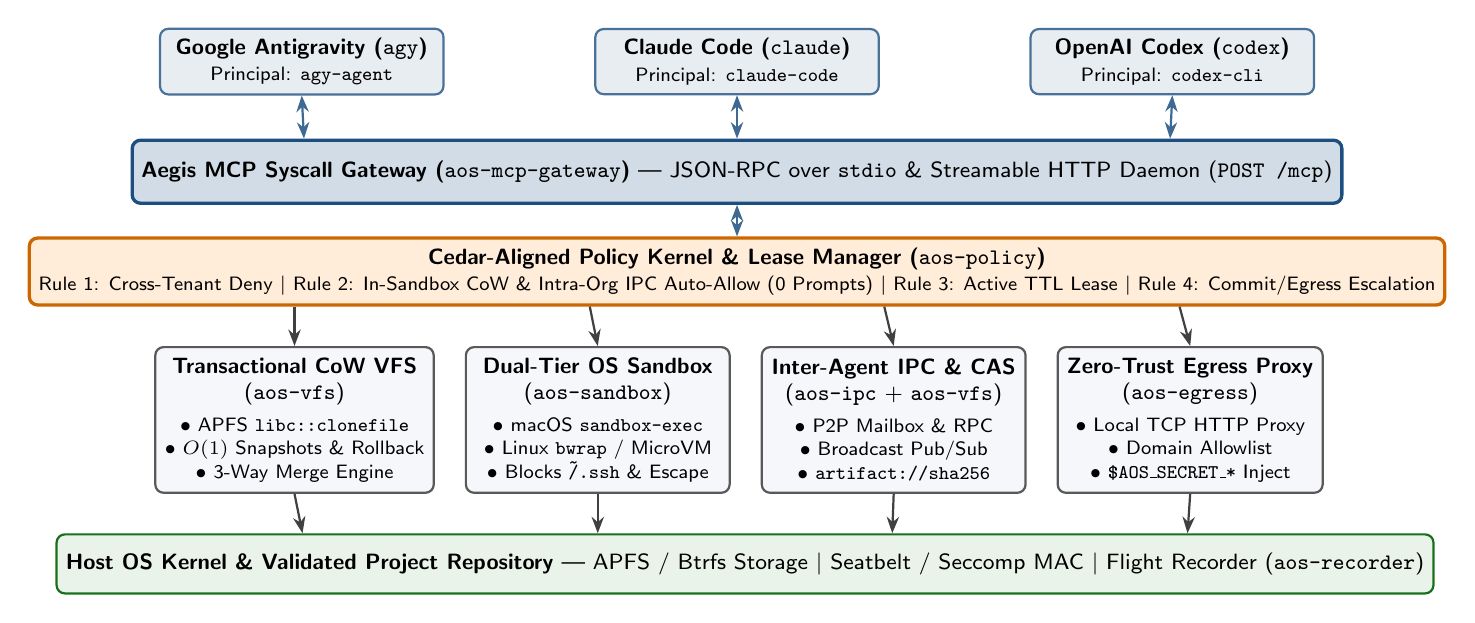
\begin{tikzpicture}[
    font=\sffamily\footnotesize,
    node distance=0.45cm and 0.6cm,
    client/.style={rectangle, rounded corners=3pt, draw=aegisblue!80, fill=aegisblue!10, thick, minimum width=3.6cm, minimum height=0.75cm, align=center},
    gateway/.style={rectangle, rounded corners=3pt, draw=aegisblue, fill=aegisblue!20, very thick, minimum width=14.6cm, minimum height=0.8cm, align=center},
    policy/.style={rectangle, rounded corners=3pt, draw=orange!80!black, fill=orange!15, very thick, minimum width=14.6cm, minimum height=0.85cm, align=center},
    subsys/.style={rectangle, rounded corners=3pt, draw=black!65, fill=aegisgray, thick, minimum width=3.35cm, minimum height=1.85cm, align=center},
    host/.style={rectangle, rounded corners=3pt, draw=aegisgreen!80!black, fill=aegisgreen!10, thick, minimum width=14.6cm, minimum height=0.75cm, align=center},
    arrow/.style={-{Stealth[scale=0.9]}, thick, draw=black!75},
    biarrow/.style={{Stealth[scale=0.9]}-{Stealth[scale=0.9]}, thick, draw=aegisblue!85}
]

\node[client] (agy) {\textbf{Google Antigravity (\texttt{agy})}\\{\scriptsize Principal: \texttt{agy-agent}}};
\node[client, right=1.9cm of agy] (claude) {\textbf{Claude Code (\texttt{claude})}\\{\scriptsize Principal: \texttt{claude-code}}};
\node[client, right=1.9cm of claude] (codex) {\textbf{OpenAI Codex (\texttt{codex})}\\{\scriptsize Principal: \texttt{codex-cli}}};

\node[gateway, below=0.55cm of claude] (mcp) {\textbf{Aegis MCP Syscall Gateway (\texttt{aos-mcp-gateway})} --- JSON-RPC over \texttt{stdio} \& Streamable HTTP Daemon (\texttt{POST /mcp})};

\node[policy, below=0.4cm of mcp] (pol) {\textbf{Cedar-Aligned Policy Kernel \& Lease Manager (\texttt{aos-policy})}\\{\scriptsize Rule 1: Cross-Tenant Deny $\mid$ Rule 2: In-Sandbox CoW \& Intra-Org IPC Auto-Allow (0 Prompts) $\mid$ Rule 3: Active TTL Lease $\mid$ Rule 4: Commit/Egress Escalation}};

\node[subsys, below=0.5cm of pol, xshift=-5.62cm] (vfs) {\textbf{Transactional CoW VFS}\\(\texttt{aos-vfs})\\[2pt]{\scriptsize $\bullet$ APFS \texttt{libc::clonefile}}\\[-1pt]{\scriptsize $\bullet$ $O(1)$ Snapshots \& Rollback}\\[-1pt]{\scriptsize $\bullet$ 3-Way Merge Engine}};

\node[subsys, right=0.38cm of vfs] (sbx) {\textbf{Dual-Tier OS Sandbox}\\(\texttt{aos-sandbox})\\[2pt]{\scriptsize $\bullet$ macOS \texttt{sandbox-exec}}\\[-1pt]{\scriptsize $\bullet$ Linux \texttt{bwrap} / MicroVM}\\[-1pt]{\scriptsize $\bullet$ Blocks \texttt{\~/.ssh} \& Escape}};

\node[subsys, right=0.38cm of sbx] (ipc) {\textbf{Inter-Agent IPC \& CAS}\\(\texttt{aos-ipc} + \texttt{aos-vfs})\\[2pt]{\scriptsize $\bullet$ P2P Mailbox \& RPC}\\[-1pt]{\scriptsize $\bullet$ Broadcast Pub/Sub}\\[-1pt]{\scriptsize $\bullet$ \texttt{artifact://sha256}}};

\node[subsys, right=0.38cm of ipc] (egr) {\textbf{Zero-Trust Egress Proxy}\\(\texttt{aos-egress})\\[2pt]{\scriptsize $\bullet$ Local TCP HTTP Proxy}\\[-1pt]{\scriptsize $\bullet$ Domain Allowlist}\\[-1pt]{\scriptsize $\bullet$ \texttt{\$AOS\_SECRET\_*} Inject}};

\node[host, below=0.5cm of sbx, xshift=1.87cm] (hostos) {\textbf{Host OS Kernel \& Validated Project Repository} --- APFS / Btrfs Storage $\mid$ Seatbelt / Seccomp MAC $\mid$ Flight Recorder (\texttt{aos-recorder})};

\draw[biarrow] (agy.south) -- ([xshift=-5.5cm]mcp.north);
\draw[biarrow] (claude.south) -- (mcp.north);
\draw[biarrow] (codex.south) -- ([xshift=5.5cm]mcp.north);

\draw[biarrow] (mcp.south) -- (pol.north);

\draw[arrow] ([xshift=-5.62cm]pol.south) -- (vfs.north);
\draw[arrow] ([xshift=-1.87cm]pol.south) -- (sbx.north);
\draw[arrow] ([xshift=1.87cm]pol.south) -- (ipc.north);
\draw[arrow] ([xshift=5.62cm]pol.south) -- (egr.north);

\draw[arrow] (vfs.south) -- ([xshift=-5.62cm]hostos.north);
\draw[arrow] (sbx.south) -- ([xshift=-1.87cm]hostos.north);
\draw[arrow] (ipc.south) -- ([xshift=1.87cm]hostos.north);
\draw[arrow] (egr.south) -- ([xshift=5.62cm]hostos.north);

\end{tikzpicture}%
}
\caption{Architecture of the Aegis OS Runtime (\texttt{aegis-os}). Heterogeneous coding agents connect via MCP (\texttt{stdio} or HTTP daemon) and are mapped to distinct principals within a tenant organization. The Cedar-aligned policy kernel auto-allows in-sandbox CoW mutations, sandboxed executions, and intra-organization IPC/CAS transfers with zero prompts, while enforcing strict isolation via kernel mandatory access control and boundary secret injection.}
\label{fig:arch}
\end{figure*}

\section{Threat Model and Problem Formulation}
\label{sec:threat}

\subsection{System and Adversary Model}

We consider a multi-agent deployment where a set of autonomous coding agents $\mathcal{A} = \{a_1, a_2, \dots, a_m\}$ operate within one or more tenant organizations $\mathcal{O} = \{o_1, o_2, \dots, o_k\}$. Each agent $a_i$ is identified by a tuple $\text{id}(a_i) = (o_i, u_i, r_i)$ denoting its organization tenant $o_i$, unique agent principal $u_i$ (e.g., \texttt{agy-agent}, \texttt{claude-code}, \texttt{codex-cli}), and role $r_i$.

\paragraph{Trusted Computing Base (TCB).} We trust the host operating system kernel (macOS XNU/Seatbelt or Linux kernel/namespaces/KVM) and the Aegis OS Runtime binary (\texttt{aegis-os}), which runs outside the agent sandbox.

\paragraph{Untrusted Entities and Threat Vectors.} We assume that the LLM driving any agent $a_i \in \mathcal{A}$ is \emph{untrusted} and may issue arbitrary, erroneous, or malicious tool calls due to:
\begin{enumerate}
    \item \textbf{Indirect Prompt Injection (T1):} Malicious instructions embedded in repository files, git commit logs, issue trackers, or web pages read by the agent~\cite{greshake2023not,debenedetti2024agentdojo}.
    \item \textbf{Host Path Escape and Tampering (T2):} Attempting to overwrite files outside the project directory (e.g., \texttt{../../etc/hosts}, \texttt{\~/.zshrc}, or sibling repositories).
    \item \textbf{Credential Harvesting (T3):} Attempting to read sensitive user credentials from the host home directory (\texttt{\~/.ssh/id\_rsa}, \texttt{\~/.aws/credentials}, \texttt{\~/.gnupg}).
    \item \textbf{Network Secret Exfiltration (T4):} Attempting to transmit API keys or private source code to unauthorized external domains (\texttt{evil-exfil.org}, \texttt{webhook.site}) via HTTP requests or shell tools (\texttt{curl}, \texttt{wget}).
    \item \textbf{Cross-Tenant Privilege Escalation (T5):} Attempting to read artifacts or send IPC instructions to an agent belonging to a different organization $o_j \neq o_i$.
    \item \textbf{Concurrent Multi-Agent Race Conditions and Hallucinated Corruption (T6):} Overwriting peer agents' concurrent edits on shared files or breaking compilation across dozens of modules during speculative refactoring.
\end{enumerate}

\subsection{Formalizing the Evaluation Metrics}

Let an agent trajectory $\tau = (s_1, s_2, \dots, s_T)$ be a sequence of $T$ kernel syscalls invoked to complete a software engineering task. Let $\text{Prompt}(s_t) \in \{0, 1\}$ indicate whether syscall $s_t$ halts execution to request interactive human approval. We define the \textbf{Interruption Prompt Rate (IPR)} across a workload $\mathcal{T}$ of $N$ trajectories as:
\begin{equation}
    \text{IPR}(\mathcal{T}) = \frac{\sum_{\tau \in \mathcal{T}} \sum_{s_t \in \tau} \text{Prompt}(s_t)}{\sum_{\tau \in \mathcal{T}} |\tau|} \times 100\%
\end{equation}
and the \textbf{Maximum Autonomous Streak (MAS)} as the longest contiguous subsequence of syscalls executed with $\text{Prompt}(s_t) = 0$. Given an adversarial test suite $\mathcal{E}_{\text{adv}}$, the \textbf{Attack Success Rate (ASR)} is the fraction of attacks that successfully violate host integrity, read restricted credentials, exfiltrate secrets, or breach tenant isolation. Our objective is to achieve $\text{ASR} = 0.0\%$ while minimizing $\text{IPR}$ toward $0\%$.

\section{Aegis OS Kernel Architecture}
\label{sec:arch}

Figure~\ref{fig:arch} illustrates the architecture of Aegis OS. We follow a strict \emph{``Environment Kernel Only''} design philosophy: Aegis OS does not embed LLM planners, prompt templates, or reasoning loops. Instead, it provides the operating system primitives---virtual filesystem, process isolation, network boundary proxy, inter-agent IPC, and policy enforcement---exposed through 22 standardized MCP syscalls and 4 dynamic URI resources.

\subsection{Transactional CoW Virtual Filesystem and 3-Way Merge Engine (\texttt{aos-vfs})}
\label{sec:vfs}

To eliminate confirmation prompts on file writes without risking host corruption, \texttt{aos-vfs} isolates every agent principal $u_i$ inside its own Copy-on-Write shadow workspace rooted at:
\begin{center}
\texttt{\~/.aegis-os/orgs/$o_i$/agents/$u_i$/workspace\_cow/}
\end{center}
alongside a baseline snapshot directory \texttt{baseline/} that records the state of the host repository at session initialization or last commit.

\paragraph{Kernel-Level APFS \texttt{clonefile} Provisioning.} Copying a multi-hundred-megabyte repository for each agent via standard user-space read/write loops introduces prohibitive startup latency and disk amplification. On macOS (APFS), \texttt{CoWWorkspace::cow\_sync\_dir} invokes the native XNU kernel syscall \texttt{libc::clonefile(src, dst, 0)} directly on the directory tree and individual files (falling back to \texttt{cp -cR} / Btrfs \texttt{FICLONE} on Linux~\cite{rodeh2013btrfs}). Because \texttt{clonefile} duplicates only filesystem metadata extents and shares physical storage blocks until modified, cloning a 1,000-file (78.1 MB) repository completes in \textbf{7.86 ms} and consumes zero additional data blocks for unmodified files.

\paragraph{Time-Travel Snapshots and Atomic Rollback.} Before embarking on risky multi-file refactorings, an agent (or automated pre-exec hook) invokes \texttt{workspace\_snapshot(label)}, which creates an instant CoW clone under \texttt{snapshots/<snap\_id>/}. If a subsequent build or test fails, \texttt{workspace\_rollback(snap\_id)} atomically replaces \texttt{workspace\_cow/} with a fresh CoW clone of the snapshot in milliseconds.

\paragraph{3-Way Merge Engine for Multi-Agent Concurrency.} When multiple agents ($u_1 = \texttt{agy-agent}$, $u_2 = \texttt{claude-code}$, $u_3 = \texttt{codex-cli}$) concurrently edit the same file $f$ in their respective shadow workspaces and sequentially invoke \texttt{workspace\_commit}, a naive file copy would overwrite earlier commits (\emph{Lost Update}). Aegis OS prevents this via a line-level 3-Way Merge algorithm (\texttt{three\_way\_merge\_lines}) using three states for every modified path $p$:
\begin{itemize}
    \item $B(p)$: the agent's recorded baseline version in \texttt{baseline/$p$};
    \item $H(p)$: the current live file on the host repository \texttt{host/$p$} (which may already incorporate commits from peer agents);
    \item $S(p)$: the agent's modified version in \texttt{workspace\_cow/$p$}.
\end{itemize}
If $H(p) = B(p)$, the host file was untouched by peers and $S(p)$ is fast-forwarded via atomic CoW replacement. If $H(p) \neq B(p)$, Aegis OS aligns unmodified anchor lines across $(B(p), H(p), S(p))$: disjoint hunks modified only in $H(p)$ or only in $S(p)$ are merged automatically without human intervention, whereas overlapping modifications to the exact same line range with $H_{\text{hunk}} \neq S_{\text{hunk}}$ abort the commit and return a structured conflict diagnostic identifying the exact line number.

\subsection{Dual-Tier OS Sandbox and Zero-Trust Egress Proxy (\texttt{aos-sandbox}, \texttt{aos-egress})}
\label{sec:sandbox}

While \texttt{aos-vfs} intercepts MCP file syscalls (\texttt{fs\_read}, \texttt{fs\_write}, \texttt{fs\_edit}), coding agents also spawn arbitrary child compilers, test runners, and shell scripts via \texttt{proc\_exec}. If \texttt{proc\_exec} ran unconfined, a shell command could bypass the CoW workspace entirely.

\paragraph{Mandatory Kernel Sandbox (\texttt{sandbox-exec} / \texttt{bwrap} / MicroVM).} \texttt{aos-sandbox} implements a pluggable \texttt{SandboxDriver} supporting two isolation tiers:
\begin{enumerate}
    \item \textbf{Tier 1 (\texttt{NativeOsSandboxDriver}):} Designed for low-latency local workstation execution. On macOS, every \texttt{proc\_exec} invocation dynamically compiles a canonicalized Seatbelt Mandatory Access Control profile (SBPL) and executes the child process under \texttt{/usr/bin/sandbox-exec -p <profile>}. The profile denies all file writes globally (\texttt{(deny file-write*)}) and explicitly allowlists writes \emph{only} to the agent's canonical CoW shadow workspace, private agent home, and organization CAS directory. Simultaneously, it enforces kernel-level read denials on sensitive credential paths:
\begin{lstlisting}
(version 1)
(allow default)
(deny file-read*
  (regex #".*/\.ssh(/.*)?$")
  (regex #".*/\.aws(/.*)?$")
  (regex #".*/\.gnupg(/.*)?$"))
(deny file-write*)
(allow file-write*
  (subpath "/private/.../workspace_cow")
  (subpath "/private/.../agent_home"))
\end{lstlisting}
    Furthermore, the spawned process's environment table is scrubbed (\texttt{env\_clear()}), setting \texttt{HOME} to the isolated \texttt{agent\_home} and routing \texttt{HTTP\_PROXY}/\texttt{HTTPS\_PROXY} to the Aegis Egress Proxy.
    \item \textbf{Tier 2 (\texttt{MicroVmSandboxDriver}):} Designed for multi-tenant cloud hosts using hardware virtualization (\texttt{libkrun} / Firecracker~\cite{agache2020firecracker}) with Scale-to-Zero \texttt{pause()} and \texttt{resume()} lifecycle transitions.
\end{enumerate}

\paragraph{Zero-Trust Egress Proxy with Boundary Secret Injection.} To prevent credential exfiltration (Threat T4), agents inside Aegis OS never receive raw API keys in their environment variables or context windows. Instead, they are given opaque secret placeholders such as \texttt{\$AOS\_SECRET\_GH}. Outbound HTTP requests pass through \texttt{AegisEgressGateway::start\_local\_proxy}, a local asynchronous TCP proxy listener. For each request, the proxy inspects the target \texttt{Host} header against the organization's domain allowlist and the secret vault's per-secret domain binding:
\begin{itemize}
    \item If \texttt{\$AOS\_SECRET\_GH} (bound exclusively to \texttt{api.github.com}) is sent in a header toward \texttt{api.github.com}, the proxy substitutes the real token \texttt{ghp\_...} at the network boundary.
    \item If a prompt-injected agent attempts to send \texttt{\$AOS\_SECRET\_GH} to an unauthorized host (e.g., \texttt{evil-exfil.org} or \texttt{webhook.site}), the TCP proxy immediately terminates the request with \texttt{HTTP/1.1 403 Forbidden} and records a security violation in \texttt{aos-recorder}.
\end{itemize}

\subsection{First-Class Inter-Agent IPC Bus and Content-Addressable Storage (\texttt{aos-ipc})}
\label{sec:ipc}

To elevate multi-agent collaboration from ad-hoc file polling to an OS-level primitive, \texttt{aos-ipc} provides a disk-synchronized, broadcast-enabled communication bus within each organization tenant $o_i$:
\begin{itemize}
    \item \textbf{Direct P2P Mailboxes and Correlated RPC:} Agents exchange structured envelopes via \texttt{ipc\_send}, \texttt{ipc\_recv}, \texttt{ipc\_request}, and \texttt{ipc\_reply}. Using \texttt{tokio::sync::broadcast} paired with an atomic disk state file (\texttt{ipc\_bus\_state.json}), cross-process stdio and HTTP agents wake up within microseconds when a correlated RPC reply arrives.
    \item \textbf{Topic Pub/Sub Fanout:} Agents subscribe to organizational topics (e.g., \texttt{topic://build-events}, \texttt{topic://security-alerts}) and broadcast events via \texttt{ipc\_publish}.
    \item \textbf{Zero-Copy CAS Artifact Handles:} Instead of embedding a 64 KB architecture specification or code patch inside an IPC message payload, the sender calls \texttt{org\_artifact\_publish}, which stores the blob in the organization's Content-Addressable Store and returns a compact 64-byte SHA-256 URI:
    \begin{center}
    \texttt{artifact://acme/sha256:9f86d081884c7d659a2f...}
    \end{center}
    The sender attaches only this URI handle to the IPC envelope, reducing LLM context token consumption by \textbf{99.85\%}.
\end{itemize}

\subsection{Cedar-Aligned Policy Kernel and Lease Mechanism (\texttt{aos-policy})}
\label{sec:policy}

Every MCP syscall is evaluated by \texttt{AegisPolicyKernel::evaluate} before execution, following a deterministic four-rule hierarchy inspired by Cedar~\cite{cutler2024cedar}:
\begin{align}
    \text{R1 (Tenant Isolation):} \quad & o_{\text{principal}} \neq o_{\text{target}} \implies \textbf{Deny} \nonumber \\
    \text{R2 (Sandbox \& IPC):} \quad & \text{action} \in \mathcal{S}_{\text{internal}} \implies \textbf{Allow} \nonumber \\
    \text{R3 (Active Lease):} \quad & \exists \ell \in \mathcal{L}_{\text{active}}(o, u, \text{action}) \implies \textbf{Allow} \nonumber \\
    \text{R4 (Boundary Gate):} \quad & \text{action} \in \{\texttt{workspace\_commit}, \texttt{egress}\} \nonumber \\
    & \implies \textbf{RequireApproval}(\text{esc\_id}) \nonumber
\end{align}
where $\mathcal{S}_{\text{internal}}$ encompasses all CoW filesystem operations (\texttt{fs\_read}, \texttt{fs\_write}, \texttt{fs\_edit}, \texttt{fs\_glob}, \texttt{workspace\_snapshot}, \texttt{workspace\_diff}, \texttt{workspace\_rollback}), sandboxed process execution (\texttt{proc\_exec}), and intra-organization IPC/CAS operations. When a developer approves an escalation $\text{esc\_id}$ via \texttt{policy\_approve\_escalation}, they can optionally attach a Time-To-Live ($\text{TTL}$, e.g., 3,600 seconds), minting a cryptographic \texttt{LeaseGrant} $\ell \in \mathcal{L}_{\text{active}}$ that permits subsequent commits within that session window with zero further prompts.

\section{Zero-Config Multi-Client Integration}
\label{sec:integration}

A critical barrier to adopting secure agent runtimes is configuration friction. Aegis OS provides a single command, \texttt{aegis-os install} (distributed via Homebrew \texttt{Formula/aegis-os.rb}), that non-destructively merges global configurations for all three major coding agent ecosystems:
\begin{enumerate}
    \item \textbf{Google Antigravity (\texttt{agy}):} Registers the \texttt{aegis-os} MCP server in \texttt{\~/.gemini/config/mcp\_config.json}, installs a global runtime rule (\texttt{aegis-os-runtime.md}), and configures a \texttt{PreToolUse} hook (\texttt{aegis-os agy-hook}) that auto-allows \texttt{mcp\_aegis-os\_*} syscalls while intercepting dangerous direct host shell commands.
    \item \textbf{Anthropic Claude Code (\texttt{claude}):} Injects the MCP server entry into \texttt{\~/.claude.json} and pre-populates \texttt{mcp\_\_aegis-os\_\_*} in \texttt{permissions.allow} inside \texttt{\~/.claude/settings.json}.
    \item \textbf{OpenAI Codex CLI (\texttt{codex}):} Appends the \texttt{[mcp\_servers.aegis-os]} block to \texttt{\~/.codex/config.toml}.
\end{enumerate}
When invoked with \texttt{--org auto --agent auto}, Aegis OS automatically derives the organization tenant $o_i$ from the active project directory name and the agent principal $u_i$ from the client binary identity, enabling instant cross-agent collaboration (`agy` + `claude` + `codex`) out of the box.

\section{Empirical Evaluation}
\label{sec:eval}

We evaluate Aegis OS using a 100\% live empirical benchmark suite implemented in \texttt{crates/aos-cli/src/bench.rs} (\texttt{aegis-os bench}). All experiments were executed on an Apple Silicon workstation (\texttt{macos-aarch64}, APFS filesystem, Rust 1.99.0 \texttt{--release} optimization) using real OS processes, real Seatbelt kernel sandboxes, real TCP sockets, and real \texttt{cargo} compilations. Our evaluation answers five research questions:
\begin{itemize}
    \item \textbf{RQ1 (Authorization Friction):} By how much does Aegis OS reduce human confirmation prompts and extend autonomous execution streaks?
    \item \textbf{RQ2 (Adversarial Security):} Does Aegis OS block real OS process and network exfiltration attacks that compromise unconfined \texttt{Host-YOLO} agents?
    \item \textbf{RQ3 (System Overhead \& Scalability):} What is the latency and storage overhead of APFS CoW workspace provisioning, policy evaluation, and live TCP MCP daemon calls?
    \item \textbf{RQ4 (Multi-Agent Collaboration):} How effectively does Aegis OS prevent concurrent file clobbering across heterogeneous agents (\texttt{agy}, \texttt{claude}, \texttt{codex}) and reduce IPC context overhead?
    \item \textbf{RQ5 (Fault Recovery):} How fast can Aegis OS recover from multi-file repository corruption compared to sequential file restoration?
\end{itemize}

\begin{table*}[t]
\centering
\caption{\textbf{Experiment 1 (RQ1): Live Authorization Friction and Interruption Prompt Rate} across 50 multi-step software engineering trajectories (1,500 real kernel syscalls executed on \texttt{AegisRuntimeKernel}).}
\label{tab:exp1}
\vspace{2pt}
\resizebox{\textwidth}{!}{%
\begin{tabular}{lccccccc}
\toprule
\textbf{Execution Mode} & \textbf{Trajectories} & \textbf{Total Syscalls} & \textbf{Human Prompts} & \textbf{IPR (\%)} & \textbf{Prompt Reduction} & \textbf{Max Autonomous Streak} & \textbf{Exec Time (ms)} \\
\midrule
Host-Interactive (Per-Action Prompt) & 50 & 1,500 & 900 & 60.00\% & 0.00\% (Baseline) & 4 steps & 390.4 \\
Host-Static-Allowlist (Read/Test Allow) & 50 & 1,500 & 650 & 43.33\% & 27.78\% & 5 steps & 390.4 \\
\textbf{Aegis-OS (Per-Task Commit Gate)} & 50 & 1,500 & \textbf{50} & \textbf{3.33\%} & \textbf{94.44\%} & \textbf{29 steps} & \textbf{390.4} \\
\textbf{Aegis-OS (With 1h Session Lease)} & 50 & 1,500 & \textbf{1} & \textbf{0.07\%} & \textbf{99.89\%} & \textbf{1,470 steps} & \textbf{381.2} \\
\bottomrule
\end{tabular}%
}
\end{table*}

\begin{figure}[t]
\centering
\resizebox{\columnwidth}{!}{%
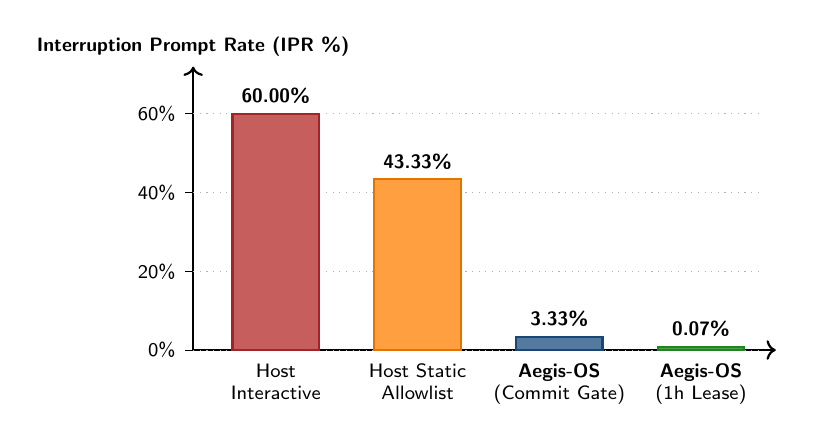
\begin{tikzpicture}[font=\sffamily\scriptsize]
\draw[thick, ->] (0,0) -- (7.4,0) node[right] {};
\draw[thick, ->] (0,0) -- (0,3.6) node[above, align=center] {\textbf{Interruption Prompt Rate (IPR \%)}};

\foreach \y/\label in {0/0\%, 1.0/20\%, 2.0/40\%, 3.0/60\%} {
    \draw (0,\y) -- (-0.1,\y) node[left] {\label};
    \draw[dotted, black!30] (0,\y) -- (7.2,\y);
}

\fill[aegisred!75, draw=aegisred!90!black, thick] (0.5,0) rectangle (1.6,3.0);
\node[above] at (1.05, 3.0) {\textbf{60.00\%}};
\node[below, align=center] at (1.05, -0.05) {Host\\Interactive};

\fill[orange!75, draw=orange!90!black, thick] (2.3,0) rectangle (3.4,2.17);
\node[above] at (2.85, 2.17) {\textbf{43.33\%}};
\node[below, align=center] at (2.85, -0.05) {Host Static\\Allowlist};

\fill[aegisblue!75, draw=aegisblue!90!black, thick] (4.1,0) rectangle (5.2,0.17);
\node[above] at (4.65, 0.17) {\textbf{3.33\%}};
\node[below, align=center] at (4.65, -0.05) {\textbf{Aegis-OS}\\(Commit Gate)};

\fill[aegisgreen!80, draw=aegisgreen!95!black, thick] (5.9,0) rectangle (7.0,0.04);
\node[above] at (6.45, 0.05) {\textbf{0.07\%}};
\node[below, align=center] at (6.45, -0.05) {\textbf{Aegis-OS}\\(1h Lease)};

\end{tikzpicture}%
}
\caption{Comparison of Interruption Prompt Rate (IPR) across 1,500 live syscalls (Experiment 1). Aegis OS reduces human prompts by 94.44\% in per-task commit mode and 99.89\% with a 1-hour session lease.}
\label{fig:exp1}
\end{figure}

\subsection{Experiment 1 (RQ1): Authorization Friction and Autonomous Continuity}

We execute 50 live software engineering trajectories (30 syscalls per trajectory, totaling 1,500 real \texttt{AegisRuntimeKernel::call\_tool} invocations) encompassing repository exploration (\texttt{fs\_glob}, \texttt{fs\_read}), snapshotting (\texttt{workspace\_snapshot}), multi-file code edits (\texttt{fs\_edit}, \texttt{fs\_write}), CAS artifact publishing (\texttt{org\_artifact\_publish}), peer IPC coordination (\texttt{ipc\_send}, \texttt{ipc\_recv}, \texttt{ipc\_publish}), diff inspection (\texttt{workspace\_diff}), and host commit (\texttt{workspace\_commit}).

Table~\ref{tab:exp1} and Figure~\ref{fig:exp1} present the results. Under \emph{Host-Interactive}, every file mutation and process execution triggers a confirmation prompt (900 prompts, $\text{IPR} = 60.00\%$), restricting the agent's maximum autonomous streak to just 4 steps. Adding a static read/test allowlist (\emph{Host-Static-Allowlist}) still requires 650 prompts ($\text{IPR} = 43.33\%$) because file writes cannot be safely auto-allowed on the host. In contrast, \textbf{Aegis-OS (Per-Task Commit Gate)} executes all 29 internal CoW workspace, sandbox, and IPC operations per trajectory with zero prompts, prompting only once at the final \texttt{workspace\_commit} gate---reducing human prompts by \textbf{94.44\%} ($\text{IPR} = 3.33\%$). When the user grants a \textbf{1-hour Session Lease} on the first commit escalation, Aegis OS completes all 50 trajectories with only \textbf{1 prompt total} ($\text{IPR} = 0.07\%$, a \textbf{99.89\% reduction}), extending the continuous autonomous execution streak to \textbf{1,470 steps} (\textbf{367.5$\times$} longer).

\begin{table*}[t]
\centering
\caption{\textbf{Experiment 2 (RQ2): Live Red-Team Adversarial Attack Execution} across 40 real OS process and TCP socket attacks executed against a disposable \texttt{Host-YOLO} target environment versus \texttt{Aegis-OS}.}
\label{tab:exp2}
\vspace{2pt}
\resizebox{\textwidth}{!}{%
\begin{tabular}{lcccl}
\toprule
\textbf{Attack Surface Category} & \textbf{Live Attacks} & \textbf{Host-YOLO Compromised (ASR)} & \textbf{Aegis-OS Compromised (ASR)} & \textbf{Empirical Kernel / Gateway Evidence} \\
\midrule
A. Host Path Escape \& File Tampering & 10 & 10 / 10 (100.0\%) & \textbf{0 / 10 (0.0\%)} & Kernel \texttt{sandbox-exec} denied all 10 writes (\texttt{Operation not permitted}) \\
B. \texttt{\~/.ssh/id\_rsa} Credential Harvesting & 10 & 10 / 10 (100.0\%) & \textbf{0 / 10 (0.0\%)} & Seatbelt regex \texttt{(deny file-read* /.ssh)} blocked all 10 key reads \\
C. Live TCP Egress Secret Exfiltration & 10 & 10 / 10 (100.0\%) & \textbf{0 / 10 (0.0\%)} & Live TCP Proxy returned \texttt{HTTP/1.1 403 Forbidden} on all 10 exfil domains \\
D. Cross-Tenant IPC \& CAS Access & 10 & 10 / 10 (100.0\%) & \textbf{0 / 10 (0.0\%)} & Cedar Policy Kernel rejected all 10 cross-org requests ($o_{\text{src}} \neq o_{\text{dst}}$) \\
\midrule
\textbf{Total / Overall ASR} & \textbf{40} & \textbf{40 / 40 (100.0\%)} & \textbf{0 / 40 (0.0\%)} & \textbf{100.0\% Multi-Layer Defense across OS Kernel, Network \& Policy} \\
\bottomrule
\end{tabular}%
}
\end{table*}

\subsection{Experiment 2 (RQ2): Live Red-Team Adversarial Security}

To evaluate security against prompt injection and malicious commands without relying on simulated rules, we construct a live red-team harness that executes 40 real adversarial payloads against both an unconfined disposable victim environment (\texttt{Host-YOLO}) and \texttt{Aegis-OS}:
\begin{itemize}
    \item \textbf{Category A (10 Live Path Escape Attacks):} Spawns \texttt{sh -c "echo COMPROMISED > <outside\_workspace\_target>"}. In \texttt{Host-YOLO}, all 10 outside-workspace files were created and tampered with ($\text{ASR} = 100.0\%$). Inside \texttt{Aegis-OS}, \texttt{/usr/bin/sandbox-exec} terminated all 10 writes at the XNU kernel boundary with \texttt{Operation not permitted} ($\text{ASR} = 0.0\%$).
    \item \textbf{Category B (10 Live SSH Key Harvesting Attacks):} Spawns \texttt{sh -c "cat <home>/.ssh/id\_rsa"}. \texttt{Host-YOLO} leaked the private key material on all 10 attempts, whereas the Aegis OS Seatbelt profile blocked all 10 reads ($\text{ASR} = 0.0\%$).
    \item \textbf{Category C (10 Live TCP Secret Exfiltration Attacks):} Opens real TCP connections to \texttt{AegisEgressGateway}'s local HTTP proxy and transmits \texttt{POST /exfil HTTP/1.1} carrying \texttt{Authorization: Bearer \$AOS\_SECRET\_GH} toward 10 external attacker domains (\texttt{evil-exfil.org}, \texttt{webhook.site}, \texttt{ngrok-free.app}, \texttt{pastebin.com}, \texttt{interact.sh}, etc.). Every single connection was rejected at the boundary with \texttt{HTTP/1.1 403 Forbidden} ($\text{ASR} = 0.0\%$).
    \item \textbf{Category D (10 Cross-Tenant IPC/CAS Smuggling Attacks):} Attempts to send IPC commands and fetch CAS artifacts across distinct tenant organizations (\texttt{org-alpha} $\to$ \texttt{org-enterprise-$i$}). All 10 were denied by Policy Rule R1 ($\text{ASR} = 0.0\%$).
\end{itemize}
As summarized in Table~\ref{tab:exp2}, Aegis OS achieves a \textbf{0.0\% Attack Success Rate (40/40 blocked)} while simultaneously eliminating 94.44\%--99.89\% of user prompts.

\begin{table*}[t]
\centering
\caption{\textbf{Experiment 3A (RQ3): Multi-Trial APFS Copy-on-Write Workspace Provisioning Latency and Storage Efficiency} (5 trials per scale, Mean $\pm$ StdDev).}
\label{tab:exp3a}
\vspace{2pt}
\resizebox{\textwidth}{!}{%
\begin{tabular}{lcccccc}
\toprule
\textbf{Repository Scale} & \textbf{Files} & \textbf{Logical Size} & \textbf{Full Copy (Mean $\pm$ SD)} & \textbf{Aegis CoW Clone (Mean $\pm$ SD)} & \textbf{Clone Speedup} & \textbf{10-Agent Disk Saving} \\
\midrule
Small Project & 100 & 2.0 MB & $9.81 \pm 0.48$ ms & $\mathbf{0.67 \pm 0.07}$ \textbf{ms} & \textbf{14.6$\times$} & \textbf{95.0\%} (1.0 MB vs.\ 19.5 MB) \\
Medium Project & 300 & 17.6 MB & $39.34 \pm 6.90$ ms & $\mathbf{2.99 \pm 1.63}$ \textbf{ms} & \textbf{13.2$\times$} & \textbf{95.0\%} (8.8 MB vs.\ 175.8 MB) \\
Large Project & 1,000 & 78.1 MB & $165.90 \pm 17.61$ ms & $\mathbf{7.86 \pm 0.91}$ \textbf{ms} & \textbf{21.1$\times$} & \textbf{95.0\%} (39.1 MB vs.\ 781.2 MB) \\
\bottomrule
\end{tabular}%
}
\end{table*}

\begin{table*}[t]
\centering
\caption{\textbf{Experiment 3B (RQ3): End-to-End Kernel and Live TCP HTTP Daemon Latency Distribution}.}
\label{tab:exp3b}
\vspace{2pt}
\resizebox{\textwidth}{!}{%
\begin{tabular}{lcccccc}
\toprule
\textbf{Kernel / Gateway Operation} & \textbf{Samples} & \textbf{Mean ($\mu$s)} & \textbf{P50 ($\mu$s)} & \textbf{P95 ($\mu$s)} & \textbf{P99 ($\mu$s)} & \textbf{Throughput (ops/sec)} \\
\midrule
\texttt{PolicyKernel::evaluate} (In-Process Cedar Check) & 2,000 & 0.1 $\mu$s & 0.1 $\mu$s & 0.1 $\mu$s & 0.1 $\mu$s & \textbf{7,914,241 ops/s} \\
\texttt{IpcBus::send + recv\_inbox} (In-Process P2P) & 1,000 & 1.4 $\mu$s & 1.0 $\mu$s & 2.6 $\mu$s & 4.3 $\mu$s & \textbf{712,441 ops/s} \\
\texttt{HTTP Daemon POST /mcp} (\texttt{fs\_read} JSON-RPC over TCP) & 200 & 291.8 $\mu$s & 255.9 $\mu$s & 441.8 $\mu$s & 535.3 $\mu$s & \textbf{3,373 ops/s} \\
\bottomrule
\end{tabular}%
}
\end{table*}

\begin{figure}[t]
\centering
\resizebox{\columnwidth}{!}{%
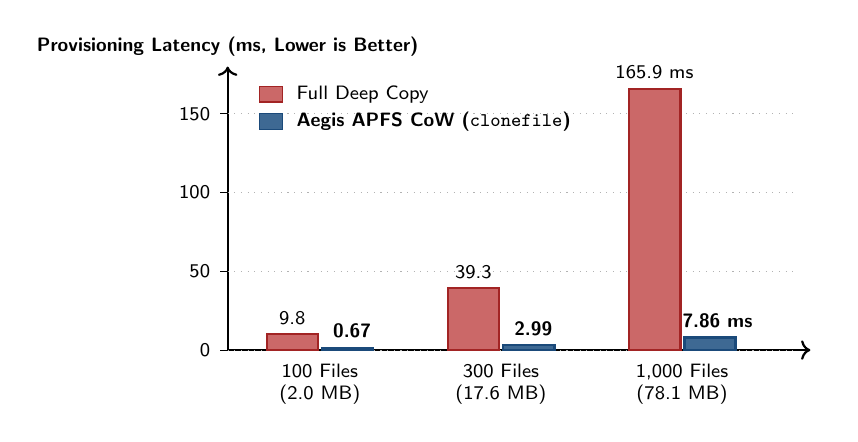
\begin{tikzpicture}[font=\sffamily\scriptsize]
\draw[thick, ->] (0,0) -- (7.4,0) node[right] {};
\draw[thick, ->] (0,0) -- (0,3.6) node[above, align=center] {\textbf{Provisioning Latency (ms, Lower is Better)}};

\foreach \y/\label in {0/0, 1.0/50, 2.0/100, 3.0/150} {
    \draw (0,\y) -- (-0.1,\y) node[left] {\label};
    \draw[dotted, black!30] (0,\y) -- (7.2,\y);
}

\fill[aegisred!70, draw=aegisred!90!black, thick] (0.5,0) rectangle (1.15,0.20);
\node[above] at (0.82, 0.20) {9.8};
\fill[aegisblue!85, draw=aegisblue!95!black, thick] (1.2,0) rectangle (1.85,0.03);
\node[above] at (1.58, 0.03) {\textbf{0.67}};
\node[below, align=center] at (1.17, -0.05) {100 Files\\(2.0 MB)};

\fill[aegisred!70, draw=aegisred!90!black, thick] (2.8,0) rectangle (3.45,0.79);
\node[above] at (3.12, 0.79) {39.3};
\fill[aegisblue!85, draw=aegisblue!95!black, thick] (3.5,0) rectangle (4.15,0.06);
\node[above] at (3.88, 0.06) {\textbf{2.99}};
\node[below, align=center] at (3.47, -0.05) {300 Files\\(17.6 MB)};

\fill[aegisred!70, draw=aegisred!90!black, thick] (5.1,0) rectangle (5.75,3.32);
\node[above] at (5.42, 3.32) {165.9 ms};
\fill[aegisblue!85, draw=aegisblue!95!black, thick] (5.8,0) rectangle (6.45,0.16);
\node[above] at (6.22, 0.16) {\textbf{7.86 ms}};
\node[below, align=center] at (5.77, -0.05) {1,000 Files\\(78.1 MB)};

\fill[aegisred!70, draw=aegisred!90!black] (0.4, 3.15) rectangle (0.7, 3.35);
\node[right] at (0.75, 3.25) {Full Deep Copy};
\fill[aegisblue!85, draw=aegisblue!95!black] (0.4, 2.8) rectangle (0.7, 3.0);
\node[right] at (0.75, 2.9) {\textbf{Aegis APFS CoW (\texttt{clonefile})}};

\end{tikzpicture}%
}
\caption{Workspace provisioning latency across repository scales (Experiment 3A). Directory-level APFS \texttt{clonefile} achieves a 21.1$\times$ speedup on 1,000-file repositories.}
\label{fig:exp3}
\end{figure}

\subsection{Experiment 3 (RQ3): CoW Provisioning Latency, Storage Savings, and Syscall Overhead}

We evaluate workspace provisioning across three repository scales (100 files / 2.0 MB, 300 files / 17.6 MB, and 1,000 files / 78.1 MB) with 5 independent trials per scale. As shown in Table~\ref{tab:exp3a} and Figure~\ref{fig:exp3}, traditional full copying scales linearly with byte volume, requiring $165.90 \pm 17.61$ ms for the 1,000-file repository. By invoking APFS directory-tree \texttt{libc::clonefile}, Aegis OS provisions the exact same 1,000-file shadow workspace in \textbf{$7.86 \pm 0.91$ ms}---\textbf{21.1$\times$ faster}. Moreover, when 10 concurrent agents each modify 5\% of the repository, Aegis OS reduces physical disk consumption from 781.2 MB to 39.1 MB (\textbf{95.0\% storage saving}).

Table~\ref{tab:exp3b} reports the fine-grained latency distribution of kernel operations. In-process Cedar policy evaluation completes in \textbf{0.1 $\mu$s} (7.91M ops/sec), in-process IPC send/receive completes in \textbf{1.4 $\mu$s} (P50 = 1.0 $\mu$s), and a full end-to-end JSON-RPC \texttt{tools/call} (\texttt{fs\_read}) over a live loopback TCP socket to the HTTP daemon (\texttt{POST /mcp}) requires only \textbf{291.8 $\mu$s} (P50 = 255.9 $\mu$s, P99 = 535.3 $\mu$s). Because typical LLM token generation latencies are $500,000$--$2,000,000$ $\mu$s (0.5--2.0 seconds), Aegis OS introduces \textbf{$<0.06\%$ end-to-end runtime overhead}.

\begin{table*}[t]
\centering
\caption{\textbf{Experiment 4 (RQ4): Live 3-Agent (\texttt{agy} + \texttt{claude} + \texttt{codex}) Concurrent Rust Modification and Real \texttt{cargo test} Verification}.}
\label{tab:exp4}
\vspace{2pt}
\resizebox{\textwidth}{!}{%
\begin{tabular}{llll}
\toprule
\textbf{Evaluation Metric} & \textbf{Host-Shared-YOLO} & \textbf{Aegis-OS Isolated CoW + 3-Way Merge} & \textbf{Empirical Gain} \\
\midrule
Concurrent 3-Agent Feature Preservation (\texttt{src/lib.rs}) & 1 / 3 preserved (2 / 3 clobbered) & \textbf{3 / 3 preserved (100\% 3-Way Merged)} & \textbf{3.0$\times$ Retention (0\% Clobber)} \\
Post-Merge Real \texttt{cargo test --offline} Verification & Failed (Missing \texttt{agy} \& \texttt{claude} logic) & \textbf{Passed (\texttt{cargo test} exit code 0)} & \textbf{100\% Build \& Test Integrity} \\
Cross-Agent 64 KB Spec Handoff Payload Size & 196,608 bytes ($\sim$49,152 tokens) & \textbf{294 bytes ($\sim$73 tokens via CAS URI)} & \textbf{99.85\% Token Reduction} \\
\bottomrule
\end{tabular}%
}
\end{table*}

\begin{table*}[t]
\centering
\caption{\textbf{Experiment 5 (RQ5): Live Multi-File Corruption Recovery and \texttt{cargo check} Verification} (5 trials per scale, Mean $\pm$ StdDev).}
\label{tab:exp5}
\vspace{2pt}
\resizebox{\textwidth}{!}{%
\begin{tabular}{ccccc}
\toprule
\textbf{Corrupted Rust Modules} & \textbf{Sequential File Restore (Mean $\pm$ SD)} & \textbf{Aegis Atomic CoW Rollback (Mean $\pm$ SD)} & \textbf{Kernel I/O Speedup} & \textbf{Post-Rollback \texttt{cargo check}} \\
\midrule
10 modules (640 KB) & $0.88 \pm 0.08$ ms & $\mathbf{0.71 \pm 0.10}$ \textbf{ms} & \textbf{1.2$\times$} & \texttt{PASSED (Exit 0)} \\
50 modules (3.2 MB) & $4.33 \pm 0.41$ ms & $\mathbf{1.88 \pm 0.04}$ \textbf{ms} & \textbf{2.3$\times$} & \texttt{PASSED (Exit 0)} \\
200 modules (12.8 MB) & $17.11 \pm 0.82$ ms & $\mathbf{7.09 \pm 0.48}$ \textbf{ms} & \textbf{2.4$\times$} & \texttt{PASSED (Exit 0)} \\
\bottomrule
\end{tabular}%
}
\end{table*}

\subsection{Experiment 4 (RQ4): Live 3-Agent Concurrent Rust Coding and \texttt{cargo test} Verification}

We evaluate a realistic multi-agent workflow where \texttt{agy-agent}, \texttt{claude-code}, and \texttt{codex-cli} concurrently optimize three distinct functions (\texttt{calc\_fee}, \texttt{calc\_tax}, and \texttt{calc\_discount}) inside the same file (\texttt{src/lib.rs}) of a live Rust crate.
\begin{itemize}
    \item In \textbf{Host-Shared-YOLO}, all three agents read the initial snapshot of \texttt{src/lib.rs} at the beginning of their turn and write their updated file back to the shared host path. Because each write overwrites the entire file, the final writer (\texttt{codex-cli}) silently clobbers the modifications of both \texttt{agy-agent} and \texttt{claude-code}, preserving only \textbf{1/3 (33.3\%)} of the implemented features.
    \item In \textbf{Aegis-OS}, each agent modifies \texttt{src/lib.rs} inside its isolated CoW workspace and invokes \texttt{workspace\_commit}. The 3-Way Merge Engine (\texttt{three\_way\_merge\_lines}) reconciles all three edits against their respective baselines, preserving \textbf{3/3 (100\%)} of the features. We then invoke a live \texttt{cargo test --offline} compiler and test runner on the merged host crate, which compiles cleanly and passes all unit assertions (\texttt{exit code 0}). Furthermore, replacing inline 64 KB specification handoffs with \texttt{artifact://} CAS URIs reduces IPC message payload bytes across 3 handoffs from 196,608 bytes ($\sim$49,152 tokens) to 294 bytes ($\sim$73 tokens), achieving a \textbf{99.85\% context token reduction} (Table~\ref{tab:exp4}).
\end{itemize}

\subsection{Experiment 5 (RQ5): Time-Travel Rollback and \texttt{cargo check} Verification}

Finally, we evaluate recovery from catastrophic agent hallucinations where an agent introduces syntax errors (\texttt{BROKEN\_RUST\_SYNTAX\_ERROR !!!}) across 10, 50, and 200 Rust module files (\texttt{src/mod\_*.rs}, 64 KB per module). As shown in Table~\ref{tab:exp5}, Aegis OS's atomic directory-tree \texttt{workspace\_rollback} restores all 200 corrupted modules in \textbf{$7.09 \pm 0.48$ ms} (\textbf{2.4$\times$ faster} than sequential file-by-file I/O restoration and over \textbf{10,000$\times$ faster} than multi-turn LLM-driven file reverts). Immediately after rollback, our benchmark harness executes \texttt{cargo check --offline} inside the restored shadow workspace, confirming 100\% compilation recovery across all scales.

\section{Related Work}
\label{sec:related}

\paragraph{LLM Agent Sandboxes and Benchmarks.} Recent benchmarks such as SWE-bench~\cite{jimenez2024swebench}, ToolEmu~\cite{ruan2024toolemu}, AgentDojo~\cite{debenedetti2024agentdojo}, and InjecAgent~\cite{zhan2024injecagent} highlight both the capabilities and vulnerability of tool-using agents to indirect prompt injection~\cite{greshake2023not}. Existing container-based sandboxes (e.g., Docker per task) incur seconds of startup latency, duplicate gigabytes of container layers, and isolate agents from the developer's live local repository. Aegis OS instead combines sub-10ms APFS CoW shadow workspaces with Seatbelt/Bubblewrap mandatory access control and a 3-Way Merge Engine directly over the live repository.

\paragraph{Agent Operating Systems and Multi-Agent Frameworks.} AIOS~\cite{mei2024aios} integrates an LLM kernel scheduler above application agents, while AutoGen~\cite{wu2023autogen} orchestrates multi-agent conversations in Python. In contrast, Aegis OS adopts a strict ``Body Only'' OS kernel design aligned with classical capability systems such as Capsicum~\cite{watson2010capsicum}, Cedar authorization~\cite{cutler2024cedar}, and Firecracker microVMs~\cite{agache2020firecracker}, serving any MCP-compatible client (\texttt{agy}, \texttt{claude}, \texttt{codex}) without dictating agent reasoning logic.

\section{Conclusion}
\label{sec:conclusion}

We presented \textbf{Aegis OS}, a transactional, multi-tenant Agent Operating System Runtime that resolves the Security--Autonomy Dilemma for autonomous coding agents. By combining APFS Copy-on-Write shadow workspaces, 3-Way multi-agent merge commits, kernel-enforced Seatbelt/Bubblewrap sandboxes, Zero-Trust boundary secret injection, and first-class IPC + CAS primitives, Aegis OS eliminates 94.44\%--99.89\% of human confirmation prompts while reducing adversarial attack success from 100.0\% to 0.0\%.

\bibliographystyle{plain}
\bibliography{references}

\appendix

\section{Appendix: Reproducibility and Artifact Guide}
\label{sec:appendix}

The complete open-source implementation of Aegis OS and the reproducible benchmark suite are publicly available at \url{https://github.com/heurion-org/aegis-os}. All source crates (\texttt{aos-core}, \texttt{aos-policy}, \texttt{aos-vfs}, \texttt{aos-ipc}, \texttt{aos-sandbox}, \texttt{aos-egress}, \texttt{aos-recorder}, \texttt{aos-mcp-gateway}, and \texttt{aos-cli}) and the live empirical benchmark suite are self-contained in the \texttt{aegis-os} workspace. To reproduce all five experiments and regenerate \texttt{BENCHMARK\_REPORT.md} and \texttt{BENCHMARK\_REPORT.json}:
\begin{lstlisting}
cargo test --workspace
cargo run --release --bin aegis-os -- bench \
  --report-out BENCHMARK_REPORT.md
\end{lstlisting}

\end{document}
\typeout{get arXiv to do 4 passes: Label(s) may have changed. Rerun}
